\documentclass[compress,color=usenames]{beamer}

\newcommand{\mytitlenbr}{1}
\newcommand{\mytitle}{Image Archive}

%\documentclass[compress,color=usenames,handout]{beamer}

%\usepackage{pgfpages}
%\pgfpagelayout{4 on 2}[a4paper,border shrink=5mm]

\usepackage{graphicx}
\usepackage{amsfonts,amssymb}
\usepackage{latexsym}
\usepackage{mdwtab}
\usepackage{xspace}
\usepackage{tikz}
\usetikzlibrary{shapes,snakes}
\usetikzlibrary{petri}

\DefineNamedColor{named}{Periwinkle}{cmyk}{0.57,0.55,0,0}
\DefineNamedColor{named}{Plum}{cmyk}{0.50,1,0,0}
\DefineNamedColor{named}{Red}{cmyk}{0,1,1,0}

\newcommand{\mH}[1]{\textcolor{Plum}{#1}}
\newcommand{\mT}[1]{\textcolor{Periwinkle}{#1}}

\newcommand{\tup}[1]{\langle #1 \rangle}

\newcommand{\dd}{{:}}
\newcommand{\I}{\mathcal{I}}
\newcommand{\csetsc}[2]{\{#1 $\mid$ #2\}}
\newcommand{\cset}[1]{\{#1\}}

\newcommand{\CON}{\textsf{CON}\xspace}
\newcommand{\ROL}{\textsf{ROL}\xspace}
\newcommand{\IND}{\textsf{IND}\xspace}
\newcommand{\PROP}{\textsf{PROP}\xspace}
\newcommand{\lang}{\mathcal{L}\xspace}


\newcommand{\mytt}[1]{\textsf{\scriptsize{#1}}}
\newcommand{\mytts}[1]{\textsf{\scriptsize{#1}}}

%\usefonttheme{serif}

\mode<presentation>
 {
 \usetheme{lined}
 }

\setbeamertemplate{navigation symbols}{}


\newcommand{\F}{\mathop{\mathsf{F}\vphantom{a}}\nolimits}
\newcommand{\G}{\mathop{\mathsf{G}\vphantom{a}}\nolimits}
\newcommand{\X}{\mathop{\mathsf{X}\vphantom{a}}\nolimits}

\newcommand{\Blue}[1]{\textcolor{blue}{#1}}
\newcommand{\Red}[1]{\textcolor{red}{#1}}
\newcommand{\Green}[1]{\textcolor{PineGreen}{#1}}


\title[GLN y Aplicaciones]{\Huge Generaci\'on de Lenguaje Natural y Aplicaciones}
%\mH{Lecture \#\mytitlenbr:} \mytitle}

\author[Areces \& Benotti]{
 Carlos Areces y Luciana Benotti\\[1ex]
\normalsize \url{{carlos.areces, luciana.benotti}@gmail.com}}

\institute[INRIA / UNC]{
INRIA Nancy Grand Est, Nancy, France\\
Universidad Nacional de C\'ordoba, C\'ordoba, Argentina}

\date{ELiC 2010 - Buenos Aires - Argentina}

\begin{document}


\beamerdefaultoverlayspecification{}


\begin{frame}[plain]
 \titlepage
\end{frame}

\begin{frame}
\frametitle{Overview}

\begin{itemize}

\item Tree Adjoining Grammars

\begin{itemize}
\item  Weak vs. Strong Generative Capacity
\item TAGS Natural Language and Complexity
\item Lexicalization of Grammars
\end{itemize}

\item TAGs for Natural Languages

\end{itemize}
\end{frame}

\begin{frame}
\frametitle{Strong vs.\ Weak Generative Capacity}

\begin{itemize}

\item Weak generative capacity of a grammar is the set of strings or the
language, e.g.\ $0^n1^n$ for $n \geq 0$

\item Strong generative capacity is the set of structures (usually the set of
trees) provided by the grammar
\end{itemize}
\end{frame}

\begin{frame}
\frametitle{Strong vs.\ Weak Generative Capacity}

\begin{center}
\begin{tabular}{rcl@{\hspace{1cm}}c}
  S & $\rightarrow$ & NP V P & (1) \\

V P & $\rightarrow$ & V NP $\mid$ V P ADV  & (2)\\

 NP & $\rightarrow$ & David $\mid$ peanuts & (3) \\

  V & $\rightarrow$ & likes & (4)\\

ADV & $\rightarrow$ & passionately & (5)
\end{tabular}
\end{center}


L(G) = \{David likes peanuts, David likes peanuts passionately\}

\end{frame}

\begin{frame}
\frametitle{Derived Tree/Parse Tree}

\begin{center}
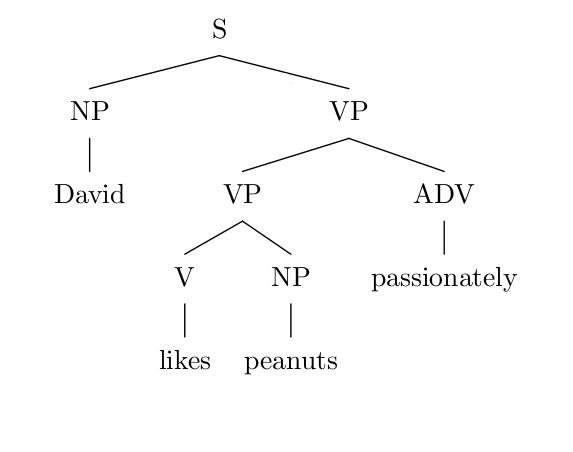
\includegraphics[scale=.4]{pics/pic2-1.jpg}
\end{center}
\end{frame}

\begin{frame}
\frametitle{Derivation Tree}

\begin{center}
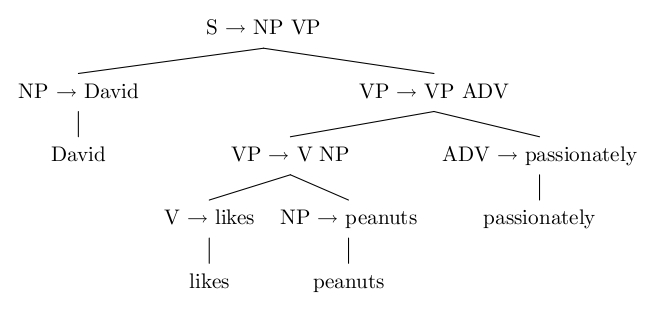
\includegraphics[scale=.4]{pics/pic2-2.jpg}
\end{center}
\end{frame}

\begin{frame}
\frametitle{Tree Sets} 

Given CFG, $G$, let $T(G)$ be the set of derived trees

\begin{center}
\begin{tabular}{rcl}
$S$ & $\rightarrow$ & $AB$\\
$A$ & $\rightarrow$ & $aA$ $\mid$ $a$\\
$B$ & $\rightarrow$ & $Bb$ $\mid$ $b$
\end{tabular}
\end{center}

\begin{center}
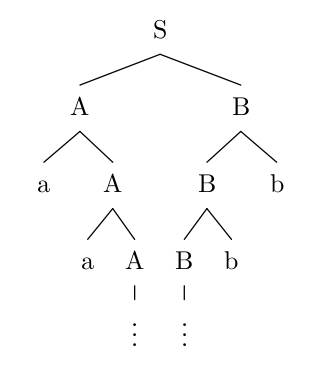
\includegraphics[scale=.3]{pics/pic2-3.jpg}
\end{center}


Tree set $T$ shown here, $T = T(G)$
\end{frame}

%\begin{frame}
%\frametitle{Tree Sets: Consider T below. There is no CFG G such that T (G) = T : Why?}


%\begin{itemize}
%\item



%S


%A


%a





%A


%A





%a





%A


%A





%A





%.


%.


%.





%b


%b





%.


%.


%.


%8




%\end{itemize}

%\end{frame}

%\begin{frame}
%\frametitle{Local Tree Predicates}

%\begin{itemize}
%\item

%A





%A $\rightarrow$ a





%A if there is a right tree context A


%A





%A $\rightarrow$ A





%b





%if there is a left tree context A





%A





%no context needed





%S





%S $\rightarrow$ A





%Apply the predicates to trees and we can accept or reject trees. That is, we


%can recognize a tree set. Just like a grammar recognizes a set of strings,


%these predicates can recognize a set of trees.


%9




%\end{itemize}

%\end{frame}

%\begin{frame}
%\frametitle{Tree Sets}

%\begin{itemize}
%\item




%S


%A


%a





%A


%A





%a





%A


%A





%A





%.


%.


%.





%b


%b





%.


%.


%.





%However, T can be recognized by a finite-state bottom-up tree automaton


%10




%\end{itemize}

%\end{frame}

%\begin{frame}
%\frametitle{Tree Sets of CFGs and Recognizable Sets}


%\begin{itemize}
%\item



%\item Recognizable Sets: Tree sets recognized by finite-state bottom-up tree


%automata: analogs of regular sets





%\item Strings sets of recognizable sets are context-free languages





%\item Recognizable sets are the same as tree sets of CFGs closed under


%relabelling homomorphisms (Thatcher, 1967)





%\item Additional strong generative power of recognizable sets by introducing


%local tree predicates


%11




%\end{itemize}

%\end{frame}

%\begin{frame}
%\frametitle{Tree Sets of CFGs and Recognizable Sets}

%\begin{itemize}
%\item




%\item Surprisingly, even context-sensitive grammars when interpreted as local


%tree predicates can only generate the recognizable sets





%\item Local sets = Tree sets for CFGs; Recognizable sets = Local sets plus


%relabeling of the nodes





%\item Hence, CSGs when interpreted as {``}filters'' on trees can only produce


%context-free languages (Peters and Ritchie, 1969; McCawley, 1967)





%\item Result can be strengthened to boolean combinations of CSG local tree


%predicates (Joshi, Levy and Yueh, 1972; Rogers, 1997)


%12




%\end{itemize}

%\end{frame}

%\begin{frame}
%\frametitle{Overview}


%\begin{itemize}
%\item



%\item Tree Adjoining Grammars


%


% Weak vs. Strong Generative Capacity


%


%


%


%TAGs  Natural Language and Complexity


%


%


% Lexicalization of Grammars





%\item TAGs for Natural Languages





%13




%\end{itemize}

%\end{frame}

\begin{frame}
\frametitle{Natural Language and Complexity}


\begin{itemize}

\item We ask the question: Does a particular formal language describe some
aspect of human language

\item Then we find out if that language isn't in a particular language class

\item For example, if we abstract some aspect of human language to the
formal language: 
$$\{ww^R \mid \mbox{ where } w \in \{a, b\}*, w^R \mbox{ is the reverse of } w\}$$ 
we can then ask if it is possible to write a regular expression for this language

\item If we can, then we can say that this particular example from human
language does not go beyond regular languages. If not, then we have to
go higher in the hierarchy (say, up to context-free languages)
\end{itemize}

\end{frame}

\begin{frame}
\frametitle{Strong vs. Weak Generative Capacity}

\begin{itemize}
\item If we consider strong generative capacity then the answer is somewhat
easier to obtain

\item For example, do we need nested dependencies to compute the
semantics in a natural way?
\end{itemize}

\end{frame}

\begin{frame}
\frametitle{Strong vs. Weak Generative Capacity}

\begin{itemize}
\item However, strong generative capacity requires a particular grammar and a
particular linguistics theory of semantics or how meaning is assigned (in
steps or compositionally)

\item So, the stronger claim will be that some aspect of human language when
you consider weak generative capacity is not regular

\item This is quite tricky: consider 
$L1 = \{a^nb^n\}$ is context-free but $L2 = \{a^*b^*\}$ is
regular and $L1 \subset L2$: so you could cheat and pick some subset of the
language which won't prove anything

\item Furthermore, the language should be infinite
\end{itemize}

\end{frame}

\begin{frame}
\frametitle{Strong vs. Weak Generative Capacity}

\begin{itemize}
\item Also, if we consider the size of a grammar then also the answer is easier
to obtain (*joyable, *richment). The CFG is more elegant and smaller
than the equivalent regular grammar:

\begin{center}
\begin{tabular}{rcl}
 V & $\rightarrow$ & X\\

 A & $\rightarrow$ & X -able $\mid$ X -ment\\

 X & $\rightarrow$ & en- NA\\

NA & $\rightarrow$ & joy $\mid$ rich\\
\end{tabular}
\end{center}

\item This is an engineering argument. However, it is related to the problem of
describing the human learning process. Certain aspects of language are
learned all at once not individually for each case.
e.g., learning enjoyment automatically if enrichment was learnt
\end{itemize}

\end{frame}

\begin{frame}
\frametitle{Is Human Language a Regular Language}

\begin{itemize}
\item Consider the following set of English sentences (strings)

\begin{itemize}
\item $S$ = If $S_1$ then $S_2$

\item $S$ = Either $S_3$, or $S_4$


\item $S$ = The man who said $S_5$ is arriving today
\end{itemize}


\item Map If, then $\rightarrow$ a and either, or $\rightarrow$ b. This results in strings like abba or
abaaba or abbaabba

\item $L = \{ww^R \mid \mbox{ where } w \in \{a, b\}^*, w^R \mbox{ is the reverse of } w\}$

\end{itemize}

\end{frame}

\begin{frame}
\frametitle{Human Language is not a Regular Language}

\begin{itemize}
\item Another example, also from English, is the set of center embedded
structures


Think of $S \rightarrow a S b$ and the nested dependencies $a_1a_2a_3b_3b_2b_1$


\item Center embedding in English:

the shares that the broker recommended were bought $\Rightarrow$ $N_1N_2V_2V_1$


the moment when the shares that the broker recommended were bought
has passed $\Rightarrow$ $N_1N_2N_3V_3V_2V_1$

\item Can you come up with an example that has four verbs and corresponding
number of nouns?
\end{itemize}

\end{frame}

\begin{frame}
\frametitle{Human Competence vs. Human Performance}

\begin{itemize}
\item What if no more than 3 or 4 center embedding structures are possible?
Then the language is finite, so the language is no longer strictly
context-free

\item The common assumption made is that human competence is
represented by the context-free grammar, but human performance suffers
from memory limitations which can be simulated by a simpler mechanism

\item The arguments about elegance, size and the learning process in humans
also apply in this case
\end{itemize}

\end{frame}

\begin{frame}
\frametitle{Human Language is not a Context-Free Language}

\begin{itemize}
\item Two approaches as before: consider strong and weak generative
capacity

\item For strong generative capacity, if we can show crossing dependencies in
a language then no CFG can be written for such a language. Why?

\item Quite a few major languages spoken by humans have crossing
dependencies:


e.g Dutch (Bresnan et al., 1982), Swiss German (Shieber, 1984), Tagalog
(Rambow and MacLachlan, 2002)
\end{itemize}

\end{frame}

\begin{frame}
\frametitle{Human Language is not a Context-Free Language}

\begin{itemize}
\item



\item Swiss German:


...


...





mer


we





em Hans


Hans-





es huus


the house-





¨


halfed


helped





aastriiche


paint





N1


N2


V1


V2


. . . we helped Hans paint the house


\item Analogous structures in English (PRO is a empty pronoun subject):


Eng: S 1 = we [V1 helped] [N1 Hans] (to do) [S 2 . . .]


SwGer: S 1 = we [N1 Hans] [S 2 . . . [V1 helped] . . .]


Eng: S 2 = PRO( ) [V2 paint] [N2 the house]


SwGer: S 2 = PRO( ) [N2 the house] [V2 paint]


Eng: S 1 + S 2 = we helped1 Hans1 PRO( ) paint2 the house2


SwGer: S 1 + S 2 = we Hans1 PRO( ) the house2 helped1 paint1



\end{itemize}

\end{frame}

\begin{frame}
\frametitle{Human Language is not a Context-Free Language}

\begin{itemize}
\item




\item Weak generative capacity of human language being greater than


context-free was much harder to show. (Pullum, 1982) was a


compendium of all the failed efforts so far.





\item (Shieber, 1985) and (Huybregts, 1984) showed this using examples from


Swiss-German:


mer d'chind


we


the children-





w





a


N1





em Hans


Hans-





es huus


the house-





¨


lond


let





¨


halfed


helped





aastriiche


paint





b


N2





x


N3





c


V1





d


V2





y


V3





. . . we let the children help Hans paint the house





\item Clear case of crossing dependencies: so cannot be handled with CFGs.


23




\end{itemize}

\end{frame}

\begin{frame}
\frametitle{The Chomsky Hierarchy}

Let $G = (N, T, P, S )$ where, $\alpha$, $\beta$, $\gamma$ $\in$ $(N \cup T)^*$

\begin{itemize}
\item unrestricted or type-0 grammars: $\alpha$ $\rightarrow$ $\beta$, such that $\alpha \not = \epsilon$

\item context-sensitive grammars: $\alpha$A$\beta$ $\rightarrow$ $\alpha$$\gamma$$\beta$, such that $\gamma \not = \epsilon$

\item context-free grammars: A $\rightarrow$ $\gamma$

\item regular grammars: A $\rightarrow$ a B or A $\rightarrow$ a

\end{itemize}

\end{frame}

\begin{frame}
\frametitle{Context-sensitive grammars:}

$L(G) = \{a^nb^n \mid n \geq 1\}$

\begin{center}
\begin{tabular}{rcl}
S & $\rightarrow$ & S BC \\

S & $\rightarrow$ & aC \\

aB & $\rightarrow$ & aa \\

C B & $\rightarrow$ & BC \\

Ba & $\rightarrow$ & aa \\

C & $\rightarrow$ & b
\end{tabular}
\end{center}

\end{frame}

\begin{frame}
\frametitle{Context-sensitive grammars:}

$L(G) = \{a^nb^n \mid n \geq 1\}$

\begin{center}
\begin{tabular}{r}
$S_1$\\
$S_2 B_1 C_1$\\
$S_3 B_2 C_2 B_1 C_1$\\
$a_3 C_3 B_2 C_2 B_1 C_1$\\
$a_3 B_2 C_3 C_2 B_1 C_1$\\
$a_3 a_2 C_3 C_2 B_1 C_1$\\
$a_3 a_2 C_3 B_1 C_2 C_1$\\
$a_3 a_2 B_1 C_3 C_2 C_1$\\
$a_3 a_2 a_1 C_3 C_2 C_1$\\
$a_3 a_2 a_1 b_3 b_2 b_1$\\
\end{tabular}
\end{center}

\end{frame}

\begin{frame}
\frametitle{Tree Adjoining Grammars}

\begin{itemize}

\item Intuition we have is that the trees produced after parsing are important for
computing the meaning.

\item So instead of building the trees using context-sensitive rules like
$\alpha A \beta  \rightarrow \alpha \gamma \beta$, we can build in the context-sensitive part into elementary
trees which is used to build larger trees.


$\Rightarrow$ Elementary trees are just like the rules in a context-free grammar.


\item The elementary trees become the basic units which can be used to
rewrite non-terminal nodes inside elementary trees.

$\Rightarrow$ This rewriting is analogous to expanding a non-terminal in a
context-free grammar.

\end{itemize}

\end{frame}

\begin{frame}
\frametitle{Arboles Finitos Ordenadios Etiquetados}

\begin{itemize}
\item Un \'arbol finito ordenado etiquetado es una estructura $t = \tup{N_t, \triangleleft_t, \prec_t, L_t}$ donde

\begin{itemize}
\item $N_t$ es un conjunto finito no vac\'io de \mH{nodos}

\item $\triangleleft_t$ y $\prec_t$ son relaciones binarias sobre $N_t$, respectivamente `dominio' (dominance) y `precedencia' (precedence)

\item $\triangleleft^t$ define un \'arbol (i.e., un \'unico nodo ra\'iz y todo nodo excepto la ra\'iz tiene un \'unico predecesor) y $\prec_t$ define un orden total sobre los hijos de un nodo. 

\item $L_t$ es la funci\'on de etiquetado, que asigna a cada nodo un conjunto de etiquetas.  
\end{itemize}
\end{itemize}
\end{frame}

\begin{frame}
\frametitle{Elementos de una TAG}

Una TAG es un conjunto finito de arboles finitos ordenados etiquetados 
con ciertas caracteristicas

\begin{columns}
\column{.65\textwidth}

\begin{itemize}
\item Tomemos dos conjuntos $V_N$ (no terminales) y $V_T$ (terminales), finitos no vac\'ios \pause

\begin{picture}(0,0)
\only<2>{
\put(175,-82){
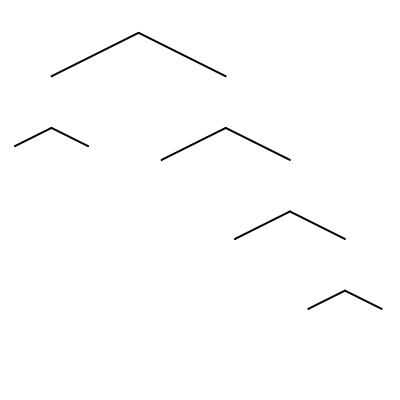
\includegraphics[scale=.5]{pics/pic2-9.jpg}
}}
\only<3>{
\put(175,-74){
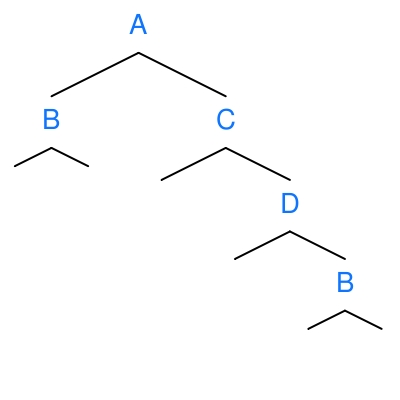
\includegraphics[scale=.5]{pics/pic2-10.jpg}
}}
\only<4>{
\put(172,-74){
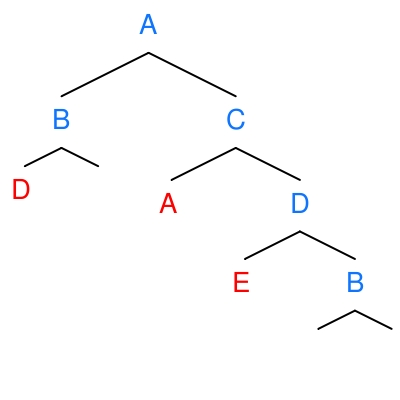
\includegraphics[scale=.5]{pics/pic2-11.jpg}
}}
\only<5>{
\put(172,-74){
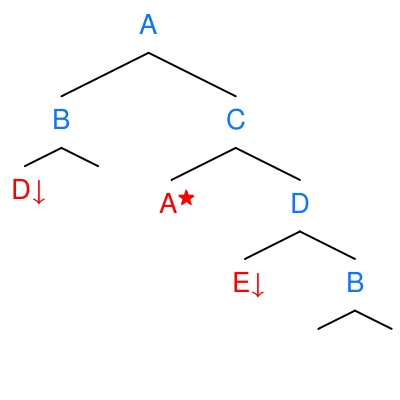
\includegraphics[scale=.5]{pics/pic2-12.jpg}
}}
\only<6>{
\put(172,-74){
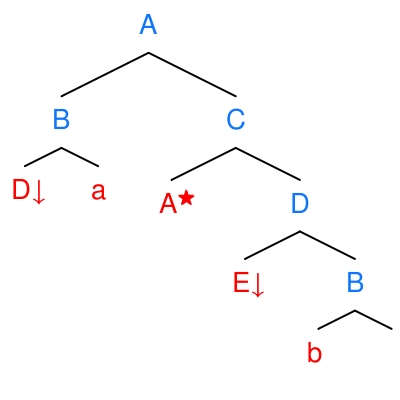
\includegraphics[scale=.5]{pics/pic2-13.jpg}
}}
\only<7>{
\put(172,-74){
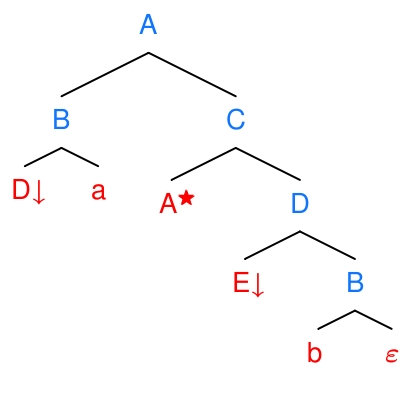
\includegraphics[scale=.5]{pics/pic2-14.jpg}
}}
\end{picture}

\vspace*{-.5cm}
\item $t = \tup{N_t, \triangleleft_t,\prec_t,L_t}$ \pause

\item $L_t$ :

\ \ \ NonLeaves$_t$ $\to$ \mH{$V_N$} \pause

\ \ \ Leaves$_t$$\to$\mH{$V_N$}$\pause\mH{\{\downarrow,\star\}}$\pause \mH{$\cup V_T$}\pause \mH{$\cup \{\epsilon\}$} 
\end{itemize}



\column{.5\textwidth}

\end{columns}
\end{frame}

\begin{frame}
\frametitle{Derivaciones en TAG}

\begin{itemize}
\item Podemos derivar nuevos arboles etiquetados mediante la aplicaci\'on de 
las operaciones de \mH{sustituci\'on} y \mH{adjunci\'on}.\pause

\item Usando \mH{\'arboles iniciales}

\begin{tabular}{l}
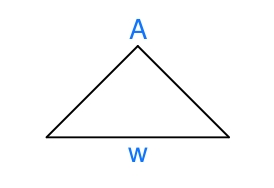
\includegraphics[scale=.5]{pics/pic2-15.jpg}
\end{tabular}
\begin{tabular}{l}
$A \in V_N$\\
$w \in (V_N\{\downarrow \} \cup V_T)^+$\pause
\end{tabular}

\item Y \mH{\'arboles auxiliares}

\begin{tabular}{l}
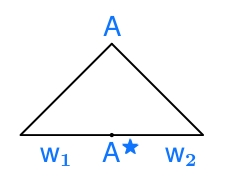
\includegraphics[scale=.5]{pics/pic2-16.jpg}
\end{tabular}
\begin{tabular}{l}
$A \in V_N$\\
$w_1,w_2 \in (V_N\{\downarrow \} \cup V_T)^+$
\end{tabular}

\end{itemize}
\end{frame}

\begin{frame}
\frametitle{Substituci\'on}

\begin{center}
\begin{tabular}{|c|c|} \hline
From & We obtain \\ \hline

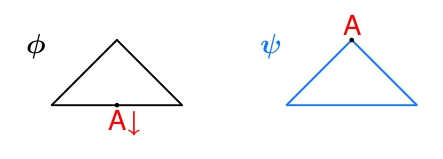
\includegraphics[scale=.4]{pics/pic2-17.jpg} & 

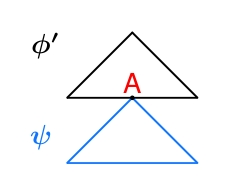
\includegraphics[scale=.4]{pics/pic2-18.jpg} \\ \hline

\multicolumn{2}{|c|}{by substituci\'on}  \\ \hline
\end{tabular}
\end{center}\pause


\mH{Ejemplo:}\begin{tabular}{l}
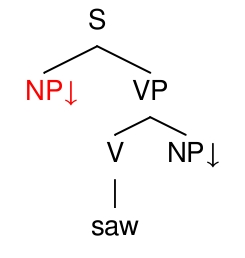
\includegraphics[scale=.4]{pics/pic2-19.jpg} \ \ \ \ \ \
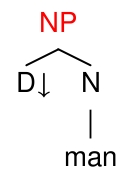
\includegraphics[scale=.4]{pics/pic2-20.jpg} \ \ \ \ \ \ 
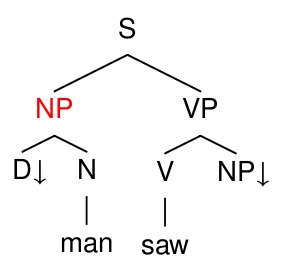
\includegraphics[scale=.4]{pics/pic2-21.jpg} 
\end{tabular}

\begin{picture}(0,0)
\put(120,40){+}
\put(190,40){$\Rightarrow$}
\end{picture}

\end{frame}


\begin{frame}
\frametitle{Tree Adjoining Grammar: Formal Definition}

\begin{itemize}

\item Tree adjoining grammar $G = (S , N, T, I, A)$ where

\begin{itemize}
\item $N$ is the set of non-terminal symbols


\item $T$ is the set of terminal symbols


\item $I$ is a set of non-recursive (terminal) trees


\item $A$ is the set of recursive (non-terminal) trees


\item $S$ is the set of start trees where $S \subseteq I$


\item $I \cup A$ is the set of elementary trees
\end{itemize}

\end{itemize}
\end{frame}

\begin{frame}
\frametitle{Tree Adjoining Grammars}

\begin{itemize}
\item Sits between context-free grammars and context-sensitive grammars

\item Handles all the weak and strong cases used to argue for the
non-context-free nature of language

\item Simple handling of crossed and nested dependencies -- compare with
context sensitive grammars

\end{itemize}
\end{frame}

\begin{frame}
\frametitle{Crossing Dependencies in TAG: $a_2a_1b_2b_1$}

\begin{center}
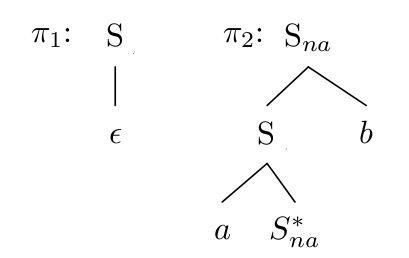
\includegraphics[scale=.4]{pics/pic2-4.jpg}
\end{center}

$$G : (T = \{a, b,\epsilon \}, N = \{S \}, I = \{\pi_1\}, A = \{\pi_2\}, S = \{\pi_1\})$$

\end{frame}

\begin{frame}
\frametitle{Crossing Dependencies in TAG: Derived Tree $a_3a_2a_1b_3b_2b_1$}

\begin{center}
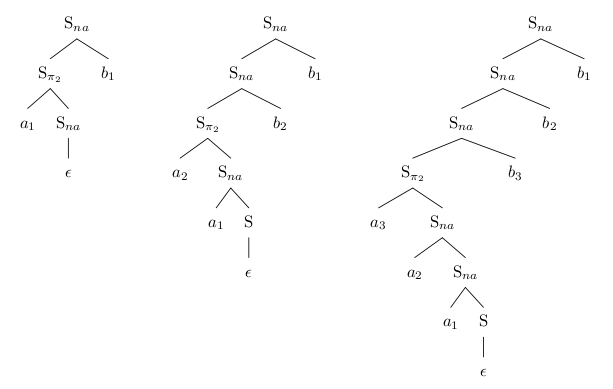
\includegraphics[scale=.4]{pics/pic2-5.jpg}
\end{center}


\end{frame}


\begin{frame}
\frametitle{Nested Dependencies in TAG: $c_1c_2d_2d_1$}


\begin{center}
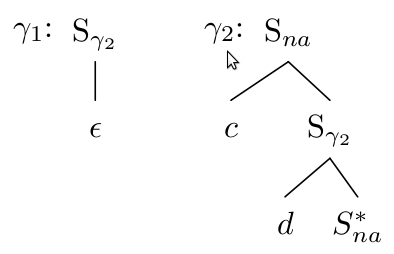
\includegraphics[scale=.4]{pics/pic2-6.jpg}
\end{center}
$$G : (T = \{c, d, \epsilon\}, N = \{S \}, I = \{\gamma_1\}, A = \{\gamma_2\}, S = \{\gamma_1\})$$


What happens if we put together a new grammar with trees $\pi_1$, $\pi_2$, $\gamma_1$, $\gamma_2$?

\end{frame}

\begin{frame}
\frametitle{Nos Ubicamos}

\begin{itemize}

\item context-sensitive grammars: $0^i$, $i$ is not a prime number and $i > 0$


\item indexed grammars: $0^n1^n2^n \ldots m^n$, for any fixed $m$ and $n \geq 0$


\item tree-adjoining grammars (TAG), linear-indexed grammars (LIG),
combinatory categorial grammars (CCG): $0^n1^n2^n3^n$, for $n \geq 0$

\item context-free grammars: $0^n1^n$ for $n \geq 0$


\item deterministic context-free grammars: $S \rightarrow S c$, $S \rightarrow S A \mid A$,
$A \rightarrow a S b \mid ab$: the language of ``balanced parentheses''


\item regular grammars: $(0\mid 1)^*00(0\mid 1)^*$

\end{itemize}

\end{frame}

\begin{frame}
\frametitle{}

\begin{center}
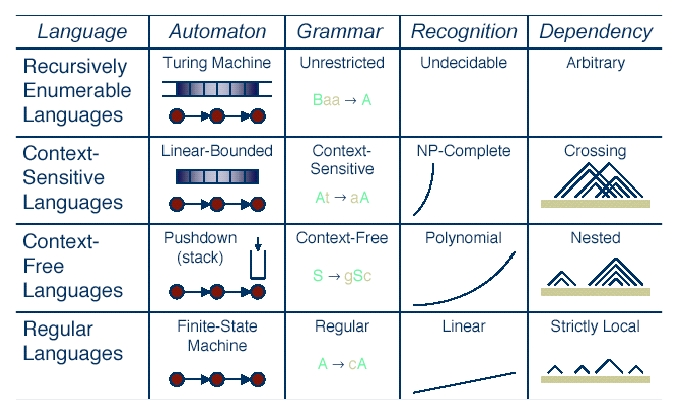
\includegraphics[scale=.4]{pics/pic2-7.jpg}
\end{center}


TAG is between CSL and CFG: has Polynomial time recognition and handles many crossing dependencies.

\end{frame}

\begin{frame}
\frametitle{}


Given grammar G and input x, provide algorithm for: Is x $\in$ L(G)?


\begin{itemize}
\item unrestricted: undecidable (grammars using {`}movement', feature structure unification)


\item context-sensitive: NSPACE[n] -- linear non-deterministic space


\item indexed grammars: NP-Complete (restricted feature structure unification)


\item tree-adjoining grammars (TAG), linear-indexed grammars (LIG), combinatory
categorial grammars (CCG), head grammars: O(n6 )


\item context-free: O(n3 )


\item deterministic context-free: O(n)


\item regular grammars: O(n)

\end{itemize}


Which class corresponds to human language?

\end{frame}

\begin{frame}
\frametitle{Tree Adjoining Grammars}

\begin{itemize}

\item Membership is in P (O(n6))


\item TALs are closed under union, concatenation, Kleene closure, h, h$-$1,
intersection with RLs and regular substitution. There is also a pumping
lemma for TALs (proofs in (VijayShanker, 1987))


Tree Adjoining Languages are a full abstract family of languages (Afl)

\item No equivalent of Ogden's Lemma. TALs are not closed under
intersection, intersection with Cfls and complementation.


\item TAGs, LIGs, CCGs, HGs (see previous slide) were shown by TAG
researchers to be weakly equivalent (VijayShanker, 1987; Weir, 1988)

\end{itemize}

\end{frame}

\begin{frame}
\frametitle{Computationally Constrained Grammar Formalisms}

\begin{itemize}


\item Why bother with computationally constrained grammar formalisms?


\item Perhaps linguists can analyze language free of any thoughts about
computational efficiency, using any system that can elegantly explain the
data

\item And then if at all necessary this analysis can be translated to a
computationally constrained formalism

\end{itemize}

\end{frame}

\begin{frame}
\frametitle{Computationally Constrained Grammar Formalisms}

\begin{itemize}

\item But what if the computational system actually provides constraints on
what can and cannot happen?

\item The linguist would be forced to assume ad-hoc restrictions to adequately
explain the facts

\item Better to start with a constrained system and grow only if necessary
(Occam's Razor)

\item Read: (Gazdar, 1981, Linguistic Inquiry) and Remarks and Replies by E.
Willams

\end{itemize}
\end{frame}


\begin{frame}
\frametitle{Lexicalization of Grammars}

\begin{itemize}

\item Why is lexicalization important? Here's a strange fact: a context-free
grammar can be infinitely ambiguous.

\item Lexicalization of a grammar means that each elementary object is
associated with some terminal symbol. This guarantees that every input
is only finitely ambiguous.

(Joshi and Schabes, 1997) show TALs are closed under lexicalization:
every TAL has a lexicalized grammar without changing the language.

\item Lexicalization is an interesting idea for syntax, semantics (in linguistics)
and sentence processing (in psycholinguistics):

What if each word brings with it an entire syntactic and semantic context
for that word?

\end{itemize}
\end{frame}

\begin{frame}
\frametitle{Lexicalization of Context-Free Grammars}

\begin{itemize}

\item Can we transform every CFG to a normal form where there is guaranteed
to be a terminal symbol on the right hand side?

\item Answer: yes -- using Griebach Normal Form

\item Every CFG can be converted to the form: $A \rightarrow a \alpha$ where $A$ is a
non-terminal, $a$ is a terminal symbol, and $\alpha \in N^*$

\end{itemize}
\end{frame}


\begin{frame}
\frametitle{Lexicalized Tree Adjoining Grammars}

\begin{itemize}

\item finite set of elementary trees, such that each tree has at least one
terminal symbol

\item Elementary trees: initial and auxiliary

\item Operations: substitution and adjunction

\item Derivation Tree: how elementary trees are put together

\item Derived Tree
\end{itemize}

\end{frame}

\begin{frame}
\frametitle{Localization of Dependencies}

\begin{itemize}

\item Syntactic:

\begin{itemize}
\item agreement: person, number, gender


\item subcategorization: sleeps (null), eats (NP); gives (NP NP)


\item filler-gap: who did John ask Bill to invite


\item word order: within and across clauses as in scrambling, clitic
movement, etc.
\end{itemize}

\end{itemize}
\end{frame}

\begin{frame}
\frametitle{Localization of Dependencies}

\begin{itemize}

\item Semantic:

\begin{itemize}
\item function-argument: all arguments of the anchoring word (the functor)
are localized


\item word clusters (flexible idioms): non-compositional, e.g. take a walk,
give a cold shoulder to


\item word co-occurences, lexical semantic aspects of meaning
\end{itemize}
\end{itemize}
\end{frame}

\begin{frame}
\frametitle{Lexicalized Tree Adjoining Grammars}

\begin{center}
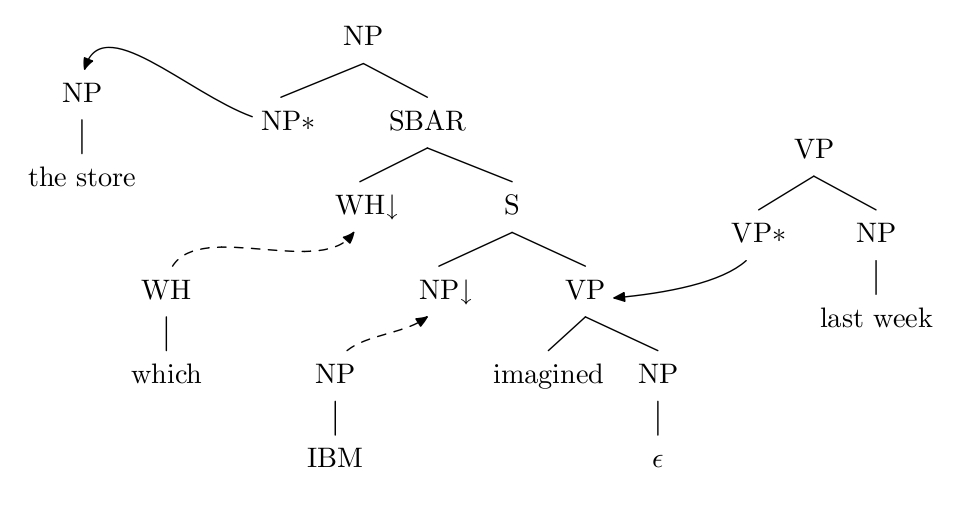
\includegraphics[scale=.4]{pics/pic2-8.jpg}
\end{center}

\end{frame}

\begin{frame}
\frametitle{La Arquitectura Estandar}

\begin{center}
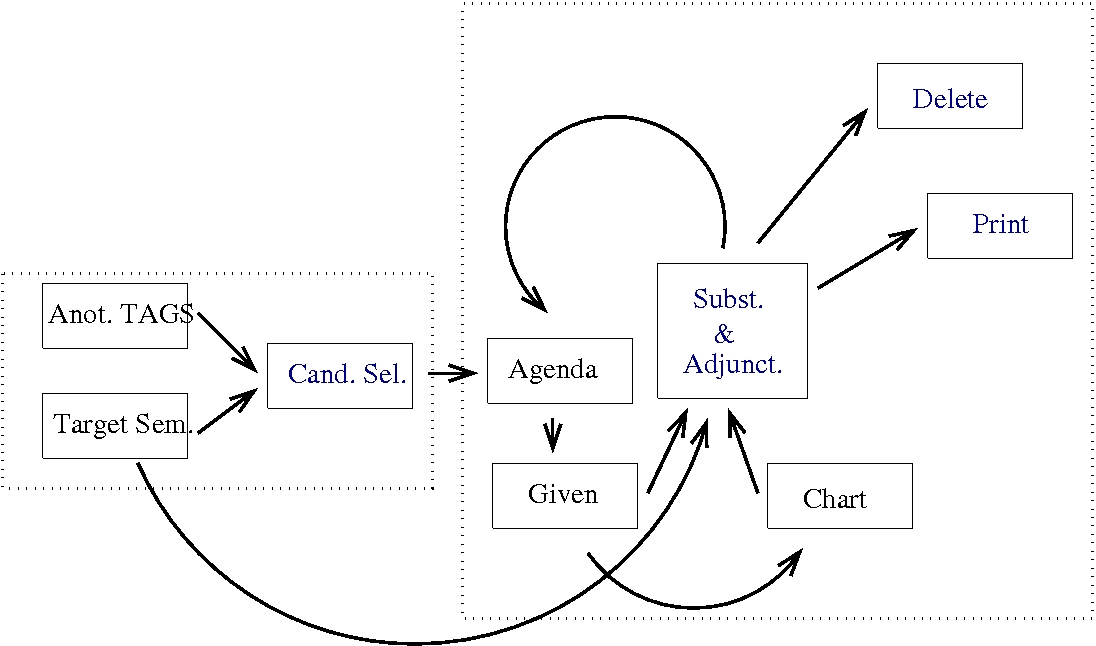
\includegraphics[scale=.32]{pics/gen.jpg}
\end{center}
\end{frame}

\end{document}
